{\bf BME154L - Spring 2012 - Exam \#2 Solutions}\hfill Name (Net ID):\underline{\hspace*{3.0in}}



\section{[70 points]}

Another approach to half-wave rectification is to utilize the ADC/DAC process instead of diodes.  We will work through this process in the following problem.  Consider a sinusoidal signal $f(t) = 5 \sin(2000 \pi t)$ V (Figure~\ref{fig:sig}(a)) and a desired output signal (a half-wave rectified input signal) (Figure~\ref{fig:sig}(b)):

\begin{figure}[htb!]
\begin{tabular}{cc}
\centering
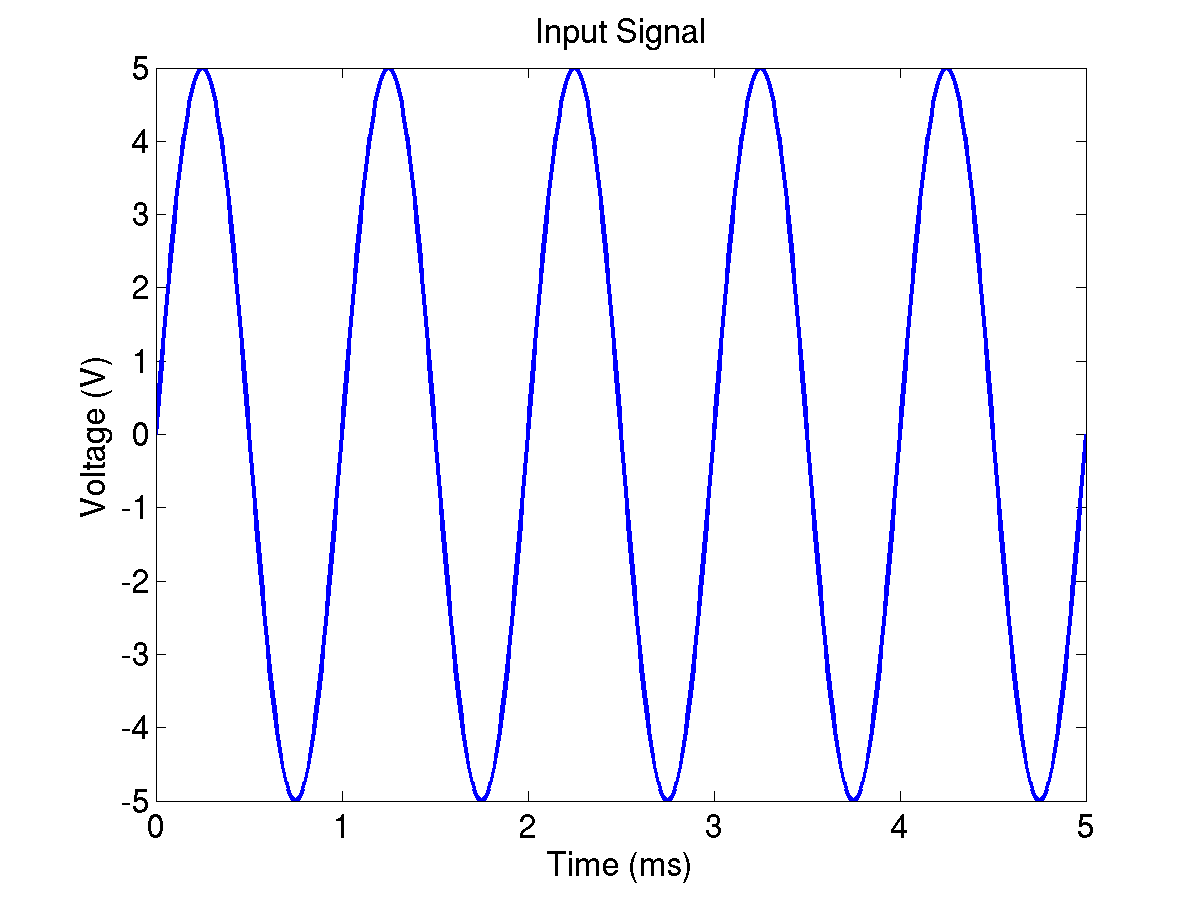
\includegraphics[width=0.5\linewidth]{in.png} &
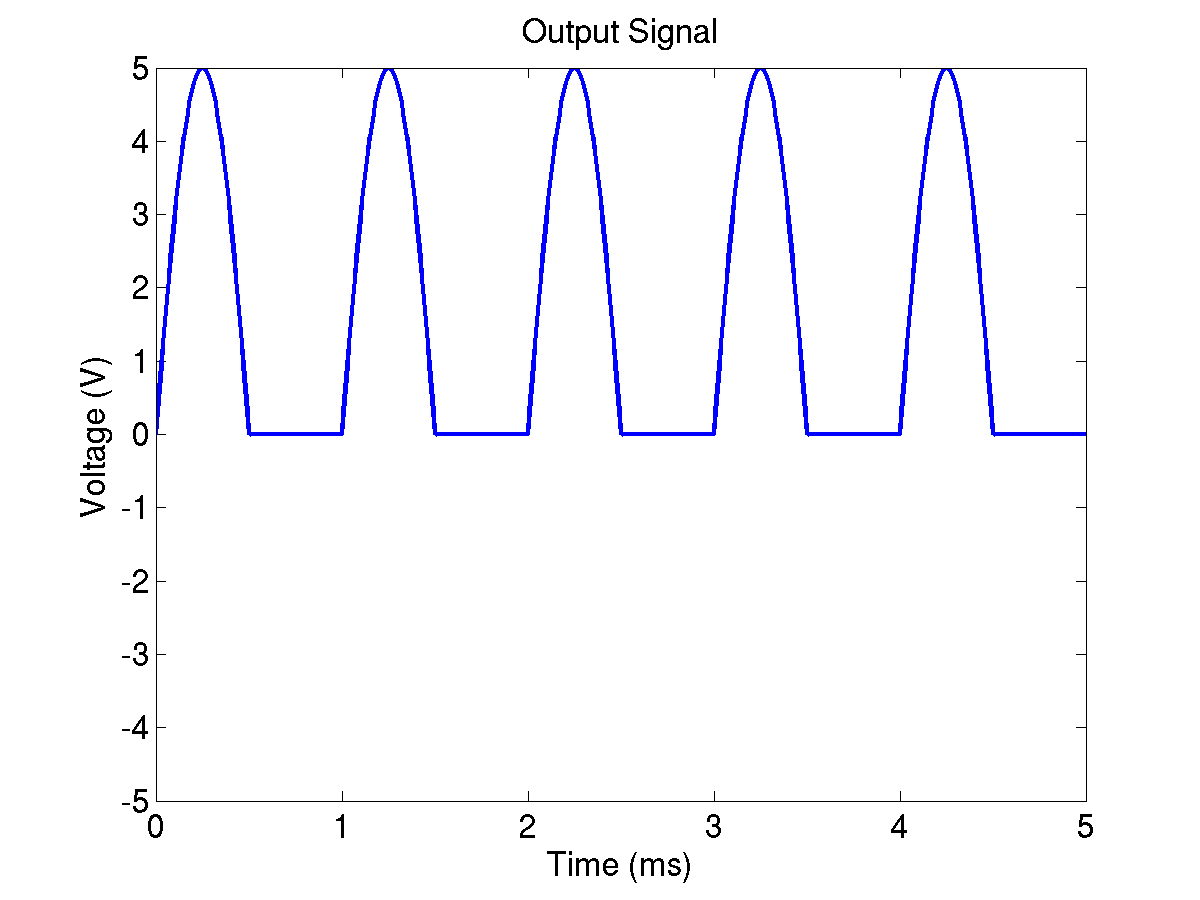
\includegraphics[width=0.5\linewidth]{out.png} \\
(a) Input Signal & (b) Output Signal \\
\end{tabular}
\caption{Input and Output Signals}
\label{fig:sig}
\end{figure}

\vspace*{0.5in}

We will use the following block diagram:

\vspace*{0.5in}

\begin{figure}[htb!]
\centering
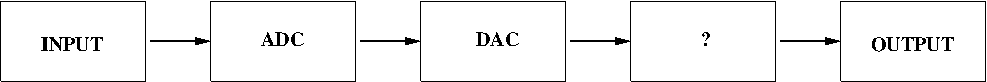
\includegraphics[width=0.75\linewidth]{block.png}
\caption{Block Diagram}
\label{fig:block}
\end{figure}

\clearpage

{\bf BME154L - Spring 2012 - Exam \#2 Solutions}\hfill Name (Net ID):\underline{\hspace*{3.0in}}



\begin{enumerate}

\item Sketch the power spectra of input (Figure~\ref{fig:sig}(a)) and output
(Figure~\ref{fig:sig}(b)) signals, labeling key features.\footnote{If you are having
trouble sketching these power spectra, then describe your thought process for
partial credit.} [10 points]

The input signal (continuous wave sinusoid) has a delta function at $f_o$ =
1000 Hz, which the output signal has harmonics at multiples of of $f_o$.  These
harmonics account for the sharper ``notches'' for the half-rectified sinusoid
at V = 0.  The way to figure this out involves recognizing that the half-wave
rectified output is the continuous sinusoidal input mutliplied by a rect that
has been convolved with a comb.  The rect convolved with a comb yields a sinc
that has been multiplied by a set of delta functions in the frequency domain,
which is then convolved with the delta function associated with the input
sinusoid.  You can plot this output power spectrum using Matlab.

\item Some sampling frequency considerations:
\begin{itemize}
    \item What is the minimum sampling frequency of the ADC that you need to
faithfully reproduce the input signal to the DAC?  [5 points]

2000 Hz

    \item What is the minimum DAC update frequency that you need to faithfully
reproduce the output signal?  Consider your answer to (a) and if there is any
benefit to updating your DAC output more frequently than the sampling frequency
of the ADC? [5 points]

There is no additional information above 1000 Hz from the ADC process, so while
the output signal has the harmonics ideally in it, having a DAC output updated
more often won't help.  

\end{itemize}

\item Given an RMS white noise voltage of 0.5 V (not shown in
Figure~\ref{fig:sig}(a)), 
\begin{itemize}
    \item What is the SNR of the input signal? [5 points]

$$ SNR = 20 * log_{10}\frac{Signal_{RMS}}{Noise_{RMS}}$$

    \item What is the ideal number of bits that should be used
to sample the input signal to generate the desired output
signal?\footnote{``Ideal'' means the number of bits needed to fully represent
the signal without wasting bits sampling just noise.}\footnote{Hint: Saturation
of an ADC can be considered a design flaw in some circuits, but it can be taken
advantage of in this problem to remove parts of your input signal that you do
not want in your output signal.} [5 points]

$$\frac{\frac{\frac{5 V}{\sqrt{2}}}{0.5 V}}{2} = 2~\textrm{bits}$$

\end{itemize}

\item Design the fastest ADC possible for this process.  Be sure to specify all
relevant component values. [10 points]

Flash ADC

Make sure that node voltages at the comparators represent voltage from 0:5 V,
in $\frac{5}{2^n -1} = 1.33 V$ increments.  Resistors needed to be in the k$\Omega$ range.

\item Successive Approximation ADC
\begin{itemize}
    \item If you were to use a successive approximation ADC for this problem, then
how many approximations would be needed for each binary number representation?  [5 points]

Number of approximations = number of bits (2)

    \item Write a general expression that relates the minimum frequency of these
successive approximations to the sampling rate of the input signal such that there is no
loss of frequency content of the input signal. [5 points]

$n$ = number of bits

$f_s$ = sampling rate

$f_{min} = n \times f_s$

\end{itemize}

\item Design an R-2R DAC for your circuit. Be sure to specify all component values.  [10 points]

See lecture notes for general form of R-2R ladder.  Make sure that the voltage source is set such that a max output voltage of 5 V is achieved, with 0 as a minimum output voltage.  There are 2 ``arms'' to this DAC, which is equal to the number of bits.

\item What error would be introduced into your DAC if the ``2R'' for your MSB
was 20\% greater than your ideal design?  (Provide a quantitative answer.) [5
points]

MSB and LSB are both affected since the current division has been skewed.  Full credit for circuit analysis showing the error on both branches.

\item Design the ``?'' block in Figure~\ref{fig:block} to achieve the desired
output signal (Figure~\ref{fig:sig}(b)).  [5 points]

Low pass filter with cutoff frequency greater than $f_{max}$ of the desired output waveform.

\end{enumerate}

\clearpage
